\section{Resultados}
\label{sec:resultados}

\begin{table}[h!b]
	\centering
	\caption{\scriptsize Tipo (origen/uso), densidad por transecto ($150m^{2}$), desviación estándar, abundancia ($\%$) y composición de resina de los desechos macroplásticos (total y por sitio de muestreo). Donde, HDPE: polietileno de alta densidad; LDPE: polietileno de baja densidad; PP: polipropileno; PS: poliestireno; EPS: poliestireno expandido; PET: tereftalato de polietileno; Nylon: poliamida seca; PE: polietileno; PVC: cloruro de polivinilo.}
	\label{tab:macroplasticos}
	\begin{tabular}{l p{2cm} l l}
		\noalign{\hrule height 1pt}
		\scriptsize Tipo de escombros               & \scriptsize N$^{\circ}$ of items per transect ($150 m^{2}$) and Standard Deviation & \scriptsize $\%$  & \scriptsize Resin                \\  \noalign{\hrule height 1pt}
		\scriptsize Bag                             & \scriptsize 166.2$\pm$252.1                                                        & \scriptsize 48.75 & \scriptsize HDPE, LDPE           \\
		\scriptsize Foodwrapper                     & \scriptsize 68.3$\pm$110.1                                                         & \scriptsize 20.05 & \scriptsize PP, PS               \\
		\scriptsize Styrofoam                       & \scriptsize 35.5$\pm$61.5                                                          & \scriptsize 10.42 & \scriptsize EPS                  \\
		\scriptsize Beverage bottle                 & \scriptsize 30.7$\pm$31.2                                                          & \scriptsize 9.00  & \scriptsize PET                  \\
		\scriptsize Fishing line                    & \scriptsize 8.5$\pm$15.7                                                           & \scriptsize 2.49  & \scriptsize Nylon                \\
		\scriptsize Bottle cap                      & \scriptsize 4.7$\pm$6.3                                                            & \scriptsize 1.37  & \scriptsize PP                   \\
		\multicolumn{4}{ l }{\scriptsize (hard)}                                                                                                                                                \\
		\scriptsize Cleaning bottle                 & \scriptsize 3.2$\pm$4                                                              & \scriptsize 0.93  & \scriptsize HDPE, PET            \\
		\scriptsize Sanitary napkin                 & \scriptsize 1.7$\pm$4.1                                                            & \scriptsize 0.49  & \scriptsize PP, PE               \\
		\scriptsize Household                       & \scriptsize 1$\pm$0.4                                                              & \scriptsize 0.29  & \scriptsize Undetermined         \\
		\multicolumn{4}{ l }{\scriptsize appliances}                                                                                                                                            \\
		\scriptsize Personal care                   & \scriptsize 0.8$\pm$2                                                              & \scriptsize 0.24  & \scriptsize PP, HDPE, PET, PDPE, \\
		\multicolumn{2}{ l }{\scriptsize container} & \multicolumn{2}{ r }{\scriptsize Varies}                                                                                                  \\
		\scriptsize Strapping band                  & \scriptsize 0.8$\pm$2                                                              & \scriptsize 0.24  & \scriptsize Polyester, PP        \\
		\scriptsize Cloth                           & \scriptsize 0.3$\pm$0.5                                                            & \scriptsize 0.10  & \scriptsize Polyester            \\
		\scriptsize Bottle label                    & \scriptsize 0.2$\pm$0.4                                                            & \scriptsize 0.05  & \scriptsize PET, PP, PVC         \\
		\scriptsize Straw                           & \scriptsize 0.2$\pm$0.4                                                            & \scriptsize 0.05  & \scriptsize PP                   \\
		\scriptsize Diaper                          & \scriptsize 0.2$\pm$0.4                                                            & \scriptsize 0.05  & \scriptsize PP, PET              \\
		\scriptsize Cigarette butt                  & \scriptsize 0.2$\pm$0.4                                                            & \scriptsize 0.05  & \scriptsize Cellulose acetate    \\
		\scriptsize Others                          & \scriptsize 15.2$\pm$19.2                                                          & \scriptsize 4.45  & \scriptsize Undetermined         \\
		\scriptsize Total                           & \scriptsize 340.8                                                                  & \scriptsize 100   & \scriptsize                      \\ \hline
		\multicolumn{4}{ l }{\scriptsize \textbf{Site}}                                                                                                                                         \\ \noalign{\hrule height 1pt}
		\scriptsize \textbf{Escondida}              & \scriptsize 52$\pm$42.4                                                            & \scriptsize 5.1   & \scriptsize                      \\
		\scriptsize \textbf{Curupí}                 & \scriptsize 190$\pm$77.1                                                           & \scriptsize 18.6  & \scriptsize                      \\
		\scriptsize \textbf{Thompson}               & \scriptsize 780$\pm$14.1                                                           & \scriptsize 76.3  & \scriptsize                      \\ \noalign{\hrule height 1pt}
	\end{tabular}
\end{table}

\subsection{Macroplásticos}
Registramos un total de 18 categorías de desechos macroplásticos (según la clasificación de la NOAA;~\cite{lippiatt2013marine}); siendo bolsa, envoltorio de alimentos, poliestireno y botella de bebida las partículas más abundantes, representando casi el $80\%$ del total (Tabla \ref{tab:macroplasticos}).

Los tres sitos de muestreo tiene fuertes diferencias en la cantidad (número de elementos) y el tipo de desechos macroplásticos (Fig. \ref{fig:macro}). Así, la playa Escondida ($4 km$ aguas arriba de la ciudad de Paraná) mostró los valores más bajos (52 macro-ítems por transecto; $150 m^{2}$), con una composición heterogénea de tipos de plástico (13 categorías diferentes) pero dominada por líneas de pesca (23 ítems). La isla Curupí (frente a la ciudad de Paraná), estuvo dominada por solo 2 tipos de macroplásticos: botellas de bebidas (81) y fragmentos de poliestireno (99). Finalmente, la playa de Thompson (ligeramente aguas abajo del outlet de Las Viejas) mostró un claro predominio de bolsas de compras (490; muchos colores y texturas diferentes) y envoltorios de alimentos (202.5), teniendo la mayor cantidad de plásticos: 757.5 artículos por transecto (es decir $5.05$ partículas macroplásticas por $m^{2}$), 14 veces más que la playa Escondida. De lejos, las resinas plásticas más abundantes fueron HDPE, LDPE, PP y PS en la playa Thompson, EPS y PET en la isla Curupí y Nylon en al playa Escondida. Se encontraron resinas de acetato de celulosa, poliéster y PVC a bajas densidades.

\begin{table}[h!t]
	\centering
	\caption{\scriptsize Tipo, densidad ($m^{2}$), derivación estándar, y abundancia ($\%$) de detritos mesoplásticos por sitio de muestreo.}
	\label{tab:mesoplasticos}
	\begin{tabular}{ p{1.2cm} l l l p{1cm} l }
		\noalign{\hrule height 1pt}
		\scriptsize Mesoplastic Type & \scriptsize Escondida & \scriptsize Curupí & \scriptsize Thompson & \scriptsize Standard deviation & \scriptsize $\%$ \\ \noalign{\hrule height 1pt}
		\scriptsize Styrofoam        & \scriptsize 47.8      & \scriptsize 35.5   & \scriptsize 16       & \scriptsize 48.3               & \scriptsize 89.3 \\
		\scriptsize Hard plastics    & \scriptsize 7.5       & \scriptsize 0      & \scriptsize 2.5      & \scriptsize 7.6                & \scriptsize 10   \\
		\scriptsize Fishing tape     & \scriptsize 0.2       & \scriptsize 0      & \scriptsize 0        & \scriptsize 0.2                & \scriptsize 0.2  \\
		\scriptsize Cassette tape    & \scriptsize 0.2       & \scriptsize 0      & \scriptsize 0        & \scriptsize 0.2                & \scriptsize 0.2  \\
		\noalign{\hrule height 1pt}
		\scriptsize Total (mean)     & \scriptsize 55.6      & \scriptsize 35.5   & \scriptsize 18.5     & \scriptsize 18.6               & \scriptsize 100  \\ \noalign{\hrule height 1pt}
	\end{tabular}
\end{table}

\subsection{Mesoplásticos}
A diferencia de los macroplásticos, los mesoplásticos tuvieron la mayor abundancia den la playa Escondida (55.6 ítems $m^{-2}$), seguida de la isla Curupí (35.5 ítems $m^{-2}$) y la playa Thompson (solo 18.5 partículas por $m^{2}$; Fig. \ref{fig:meso}). La abundancia promedio de mesoplástico estuvo cerca de 46 ítems $m^{-2}$, siendo el plástico espumado (Styrofoam) la categoría dominante (41.1 ítems $m^{-2}$) (Tabla \ref{tab:mesoplasticos}).

\begin{figure}[h!t]
	\centering
	\begin{subfigure}[b]{0.3\linewidth}
		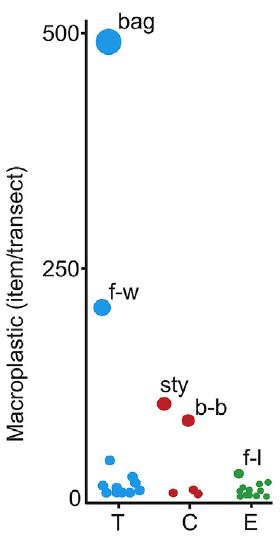
\includegraphics[width=\linewidth]{figura2/figura2a.png}
		\caption{macro-}
		\label{fig:macro}
	\end{subfigure}
	\begin{subfigure}[b]{0.3\linewidth}
		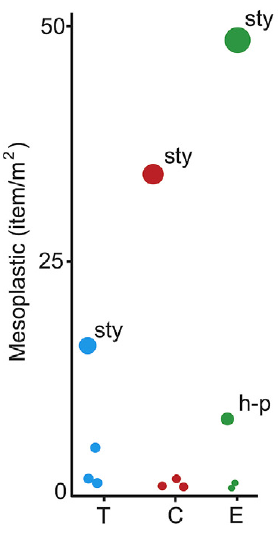
\includegraphics[width=\linewidth]{figura2/figura2b.png}
		\caption{meso-}
		\label{fig:meso}
	\end{subfigure}
	\begin{subfigure}[b]{0.3\linewidth}
		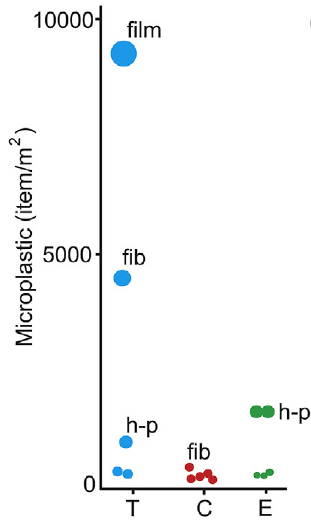
\includegraphics[width=\linewidth]{figura2/figura2c.png}
		\caption{microplástico}
		\label{fig:micro}
	\end{subfigure}
	\caption{Gráfico de burbujas que muestra las densidades en cada área de muestreo. Donde: f-w: envoltura de alimentos, pocilga: espuma de poliestireno, b-b: botella de bebida, hilo de pescar, h-p: pieza de plástico duro, fib: fibra.}
	\label{fig:densidades}
\end{figure}

\begin{table}[h!b]
	\centering
	\caption{\scriptsize Tipo, densidad ($m^{2}$), derivación estándar, y abundancia ($\%$) de detritos microplásticos por sitio de muestreo.}
	\label{tab:microplasticos}
	\begin{tabular}{ l l l l l l l }
		\noalign{\hrule height 1pt}
		\tiny               & \tiny Escondida & \tiny Curupí & \tiny Thompson & \tiny Standard deviation & \tiny $\%$ & \tiny Category  \\\hline
		\tiny Fiber         & \tiny 1431.4    & \tiny 90     & \tiny 4466.9   & \tiny 1899.6             & \tiny 33.1 & \tiny Primary   \\
		\tiny Hard plastics & \tiny 1424.2    & \tiny 18.8   & \tiny 421.7    & \tiny 51.8               & \tiny 0.9  & \tiny Secondary \\
		\tiny Styrofoam     & \tiny 33.2      & \tiny 11.3   & \tiny 36.2     & \tiny 2645.4             & \tiny 17.5 & \tiny Secondary \\
		\tiny Film          & \tiny 0         & \tiny 0.8    & \tiny 8953.5   & \tiny 6772.3             & \tiny 48.2 & \tiny Secondary \\
		\tiny Fiber-roll    & \tiny 0         & \tiny 0      & \tiny 72.9     & \tiny 54.5               & \tiny 0.4  & \tiny Primary   \\
		\noalign{\hrule height 1pt}
		\tiny Total (mean)  & \tiny 2899      & \tiny 131    & \tiny 12687    & \tiny 8548.1             & \tiny 100  & \tiny           \\ \noalign{\hrule height 1pt}
	\end{tabular}
\end{table}

\subsection{Microplásticos}
Las películas y fibras fueron los elementos dominantes en las muestras de microplásticos (Tabla \ref{tab:microplasticos}). Se encontró un promedio de 4654 fragmentos de microplásticos (por $m^{2}$) en los sedimentos de la costa de los tres muestreos (playas e islas). En la playa Thompson se registró un promedio de 12687 micropartículas $m^{-2}$  ($81\%$ del total), pero solo 131 en la isla Curupí (Fig. \ref{fig:micro}). La película y la fibra de microplástico eran extremadamente abundantes en la playa de Thompson.

El CAP (y el subsiguiente PERMANOVA) mostró diferencias significativas en la abundancia y el tipo de microplásticos entre las tres playas (sitios de muestreo)($p-valores=<0.003$; Suma de cuadrados (Q) dentro de los grupos $=2.829$)(Fig. \ref{fig:cap}).

La Tabla \ref{tab:correlaciones} muestra que los valores de densidad de las clases de tamaño (macro, meso y microplástico) no fueron sustitutos entre sí (no se detectaron correlaciones). Si bien se pudieron detectar algunas tendencias débiles (ej.: valores de alta concentración de macro y microplásticos en la playa de Thompson), no fueron estadísticamente significativas. Particularmente, la abundancia mesoplástica mostró una tendencia completamente independiente. Por ejemplo: los valores más bajos de macroplástico se encontraron en la playa Escondida, pero el mesoplástico mostró la mayor concentración en la misma playa. Mientras que las concentraciones más altas de macro y microplásticos se encontraron en la playa de Thompson, la concentración de mesoplástico fue la más baja.

\begin{table}[h!t]
	\centering
	\caption{\scriptsize Correlaciones entre los diferentes rangos de incautación de plástico.}
	\label{tab:correlaciones}
	\begin{tabular}{ p{4cm} p{2cm} l }
		\noalign{\hrule height 1pt}
		\scriptsize                      & \scriptsize $r^{2}$ & \scriptsize $p-value$ \\ \noalign{\hrule height 1pt}
		\scriptsize Macro- $vs.$ meso-p  & \scriptsize 0.006   & \scriptsize 0.85      \\
		\scriptsize Meso- $vs.$ micro-p  & \scriptsize 0.022   & \scriptsize 0.72      \\
		\scriptsize Micro- $vs.$ macro-p & \scriptsize 0.199   & \scriptsize 0.27      \\
		\noalign{\hrule height 1pt}
	\end{tabular}
\end{table}

\subsection{Ingestión de pescado}
Todos los peces estaban contaminados con al menos un microplástico. El número de elementos registrados en el tracto digestivo de \textit{P. lineatus} adulto promedió $9.9$ partículas microplásticas. El valor máximo de partículas microplásticas registradas en un individuo fue 27 (Fig \ref{fig:particulas_microplasticas}). Los tamaños de las partículas oscilaron entre $0.5$ y $3mm$ y los colores registrados fueron azul (la mayoría), negro, amarillo, rojo y transparente.

\begin{figure}[h!b]
	\centering
	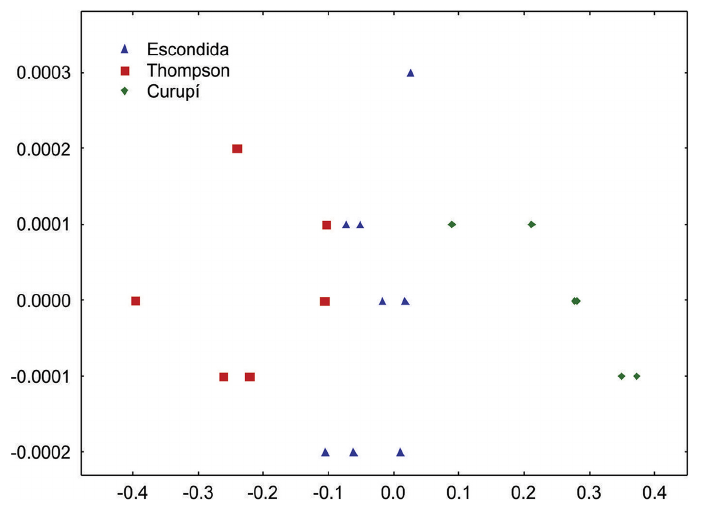
\includegraphics[width=0.5\textwidth]{figura3.png}
	\caption{Gráfica de ordenación del Análisis Canónico de Coordenadas Principales (CAP) que muestra diferencias significativas en abundancia y tipo de microplásticos entre los tres sitios de muestreo (playa Escondida, playa Thompson, isla Curupí).}
	\label{fig:cap}
\end{figure}

\begin{figure}[h!t]
	\centering
	\begin{subfigure}[b]{0.6\linewidth}
		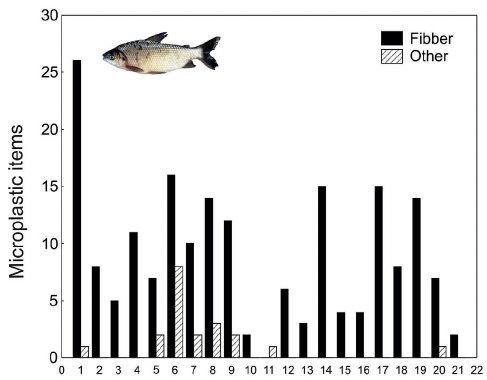
\includegraphics[width=\linewidth]{figura4/figura4a.png}
		\caption{Número de artículos}
		\label{fig:numero_articulos}
	\end{subfigure}
	\begin{subfigure}[b]{0.2\linewidth}
		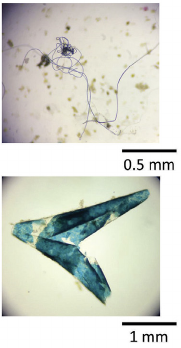
\includegraphics[width=\linewidth]{figura4/figura4b.png}
		\caption{Fibras y un trozo de película plástica}
		\label{fig:fibra_pelicula}
	\end{subfigure}
	\caption{Partículas microplásticas (fibras y otras) encontradas en el tracto digestivo de P. Lineatus.}
	\label{fig:particulas_microplasticas}
\end{figure}
